本節では、花崗岩コアを表面を伝播する弾性波計測の方法について述べる。
以下、実験に用いたコアサンプルについてはじめに述べる。
次に、強い弾性波を励起するために新たに設計、制作した圧電超音波トランスデューサの
仕様について述べた後,計測システム全体の構成、計測点(超音波の送受信位置)の配置を示す。
\subsection{実験供試体}
 超音波計測に用いた花崗岩供試体の外観と形状、大きさを、図\ref{fig:fig1}に示す。
この供試体は、岡山県万成の採石場で採取した万成花崗岩を円柱状に加工したもので、
直径約66mm, 高さは60mmである。主要造岩鉱物は石英、雲母、ナトリウムおよびカリ長石で、
結晶粒のサイズは数mmから数cm程度となっている。なお、外観からは肉眼で観察できる
き裂や欠けなどの損傷はなく、風化や造岩鉱物の明らかな変質も認められない。

 ここで、供試体内部と表面の位置を指定するための$XYZ$直交座標を図\ref{fig:fig1}の
(b)および(c)のように取る。超音波の送信と受信は、花崗岩供試体の上面$(Z=0)mm$で行い,
主として直径方向に伝播する表面波を観測する。
%--------------------
\begin{figure}[h]
	\begin{center}
	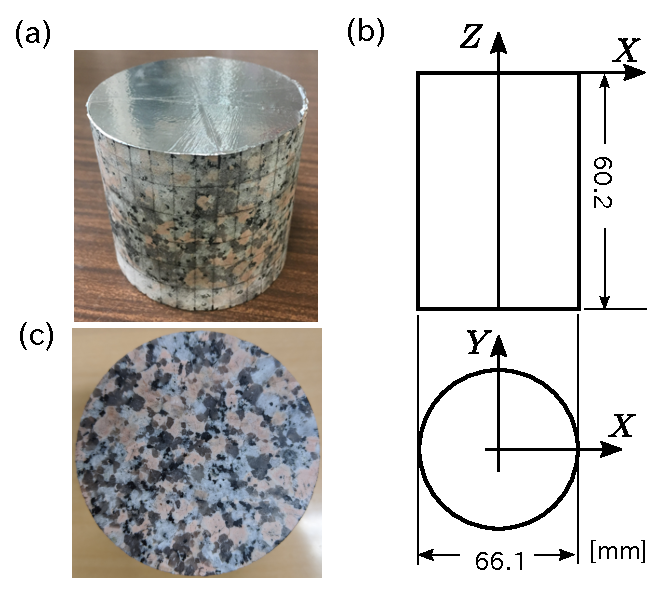
\includegraphics[width=0.6\linewidth]{Figs/fig1.eps} 
	\end{center}
	\caption{
		超音波計測に用いた花崗岩コア供試体(万成花崗岩).
	} 
	\label{fig:fig1}
\end{figure}
%--------------------
\subsection{送信用超音波トランスデューサ}
本年度は、強い超音波を励起するための接触型線集束(ラインフォーカス)・トランスデューサを
設計、制作した。ラインフォーカス・トランスデューサの構成は図\ref{fig:fig2}に示すようで
あり、圧電素子を赤、圧電素子がマウントされたシューを青で示してある。この図に示されるように、
曲率をもった圧電素子が、くさび状のポリエーテルイミドのシューに取り付けられている。
圧電素子の曲率中心は、シュー先端部にあるように設計されており、シュー先端部の幅は1mm、
圧電素子の共振周波数は2MHzで、圧電素子の厚み振動によってシュー内部に縦波を励起する.
花崗岩試料の弾性波速度が縦波で約5km/s,横波が3km/s程度であることがわかっている。
そのため、2MHzの超音波の岩石試料内部での波長は、縦波、横波それぞれ、約2.5mmと1.5mmと
見積もられる。シュー先端部の幅は、このことを踏まえ、波長以下の寸法となるよう1mmとした。
一方、圧電素子の長さは、シュー先端部の幅と、岩石中での超音波波長より十分に長くなるよう
40mmとした。これにより、線音源に近い状態をシュー先端部が試料に接触する位置で作り出し、
試料内部に平面波を励起する。完全な平面波は、距離による減衰が無く、伝播挙動も理解しやすい。
このことは、岩石のような強い散乱減衰を起こす、不均質材中の弾性波挙動を調べる上で有利
な条件であることから、今回、平面波に近い場を励起することを目的として、ラインフォーカス
トランスデューサを設計し、計測に用いることとした。
%--------------------
\begin{figure}[h]
	\begin{center}
	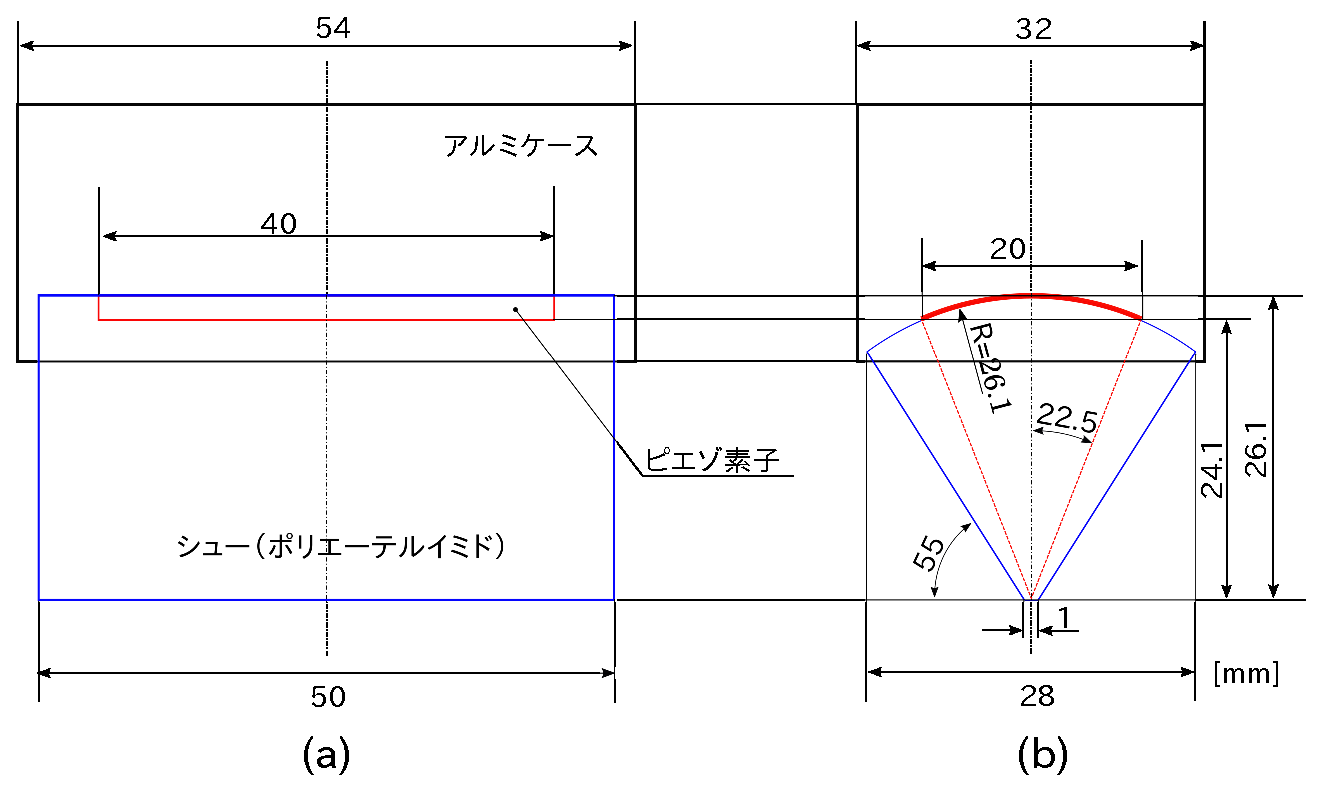
\includegraphics[width=0.8\linewidth]{Figs/fig2.eps} 
	\end{center}
	\caption{
		接触型ラインフォーカス探触子の形状と寸法.
	} 
	\label{fig:fig2}
\end{figure}
%--------------------
\begin{figure}[h]
	\begin{center}
	\includegraphics[width=0.5\linewidth]{Figs/fig2_2.eps} 
	\end{center}
	\caption{
		(a),(b)接触型ラインフォーカス探触子の外観.(c)花崗岩供試体上面への固定状況.
	} 
	\label{fig:fig2_2}
\end{figure}
%--------------------
\subsection{超音波計測系の構成}
超音波計測システムの構成を図\ref{fig:fig3}に示す。ここに示したように、花崗岩コア供試体は、
3軸ステージ上に固定して位置調整を行う。
3軸ステージは、水平xy平面で並進2軸、鉛直方向を軸とする回転1軸を持つ。
各ステージはステッピングモーターで駆動され、試料の位置と向きを正確に調整
することができる。送信に用いるラインフォーカス・トランスデューサは、コア供試体
上面($Z=0$)に,シュー先端部をグリセリンペーストのカップリング剤を使って
密着させた状態で固定する。受信には、レーザードップラー振動計
(LDV: laser Doppler vibrometer)を用いる。
LDVは、高い空間解像度と十分な周波数帯域を持つことから、ここでの計測に
理想的なものである。ただし、試料表面の状態により信号−雑音比(SN比)が大きく
変化することが欠点である。そのため、十分な反射レーザー光の受光感度を得るため、
コア供試体の上面にはアルミ箔を貼り付けている。アルミ箔は、供試体表面にオイル
を均等に塗り、供試体とアルミ箔の間に空隙を残さないように貼り付けている。
ラインフォーカス・トランスデューサは、超音波探傷試験用のパルサーレシーバで
矩形パルスを印加して励起する。また、LDVはLDVコントローラを介して制御PC
とオシロスコープに接続し、オシロスコープでは速度波形の取り込みをパルサーレ
シーバと同期させて行う。制御PCは、LDVコントローラとオシロスコープとの
通信を行い、LDVから受光感度のデータを受け取り、計測点毎にフォーカス
調整をPCからのコマンド制御で実行する。一方、オシロスコープからはLDVから
取り込み、デジタイズされた波形を取得し、保存する。なお、制御PCは、3軸ステージ
の制御も、ステージコントローラを介して行う。以上、本システムでは、LDVのフォーカス
調整実行、受光感度の記録、振動波形取り込み,3軸ステージ制御による計測点
位置調整を、PCからのシリアル通信によるコマンド制御で行い、一連の計測を自動化
している。
%--------------------
\begin{figure}[h]
	\begin{center}
	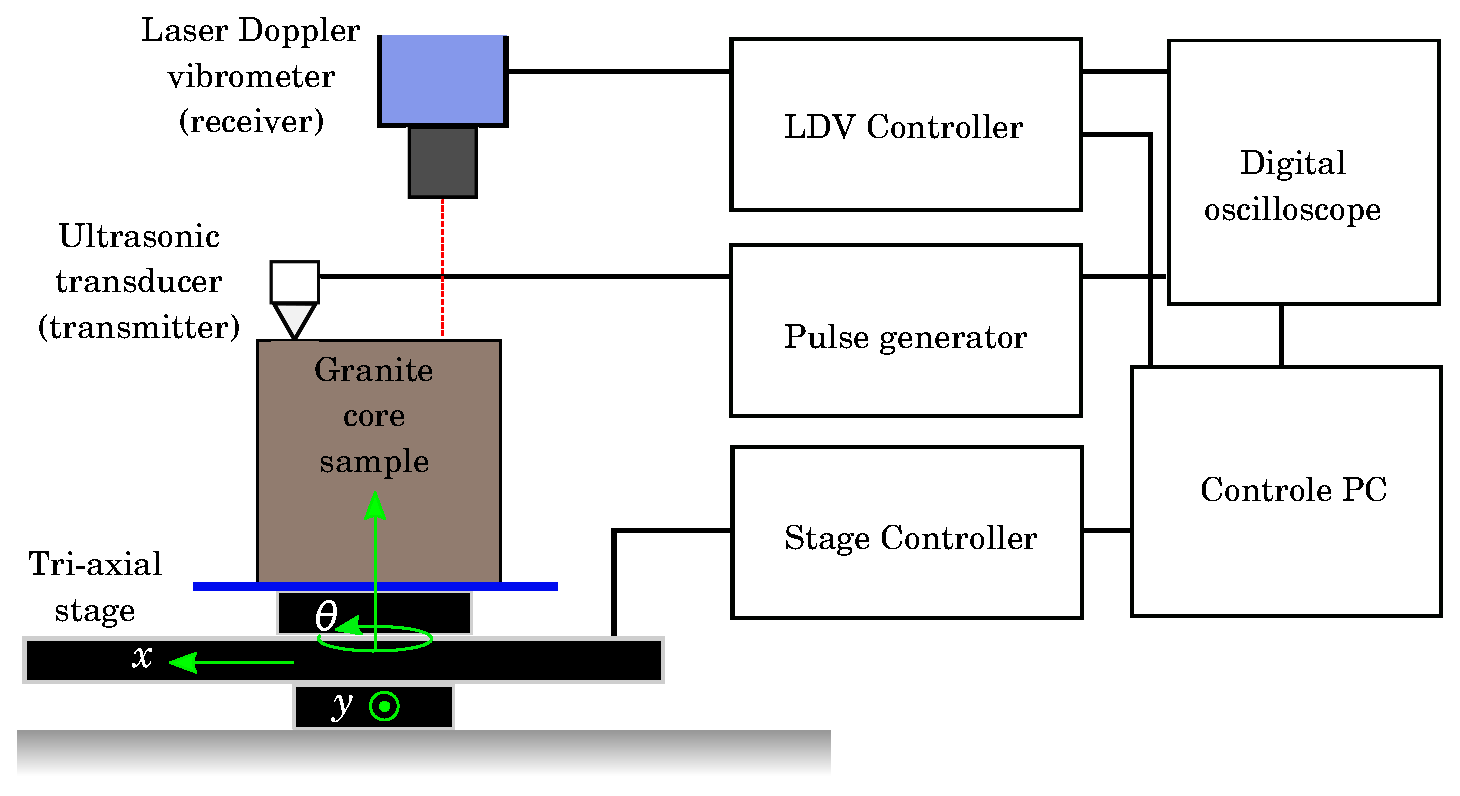
\includegraphics[width=0.8\linewidth]{Figs/fig3.eps} 
	\end{center}
	\caption{
		超音波測定装置の構成.
	} 
	\label{fig:fig3}
\end{figure}
%--------------------
\subsection{送受信点の配置}
 超音波の送受信位置を指定するために、図\ref{fig:fig4}に示す$xy$直交座標系を
供試体上面($Z=0$)にとる。$xy$座標は、$XY$座標と反時計回りの方向に$\theta$だけ
向きが異なる。ここで、$x$軸は、入射波の伝播方向に一致させるようにとる。
すなわち、X軸から測った角度$\theta$は、同時に入射波の伝播方向を表すこととする。
$\theta$方向に超音波を入射するために、ラインフォーカス・トランスデューサは、
図\ref{fig:fig4}の$\cal S$で示した位置にシュー先端部を密着させて固定する。
一方、LDVによる超音波の受信は,同図において${\cal R}$で示した測線上を、0.5mm
のピッチでスキャンして波形取得を行う。測線の長さは20mmとして、その結果、1測線あたりの
測定点数は41点となる。送信位置$\cal S$、受信位置$\cal R$は、いずれもコア供試体
中心($(x,y)=(0,0)$mm)から20mm離れた位置にとり、これにより40mmの距離
を伝播した超音波の上下動($Z$方向成分)を計測する。以上のような計測を、入射角度
$\theta$を0度から330度まで30度ピッチで行い、計12の入射方向に対して、
供試体直径方向に伝播する超音波波形を計測する。以下、送信トランスデューサの駆動に
用いるパルサーの設定、波形収録に関する条件、送受信点配置の詳細をまとめて示す。
\begin{enumerate}
\item パルサー設定
	\begin{itemize}
		\item 電圧パルス形状:矩形
		\item 印加電圧: -400V
		\item パルス幅: 0.25$\mu$sec 
		\item パルス繰り返し周波数:2kHz
	\end{itemize}
\item 波形収録条件
	\begin{itemize}
		\item サンプリング周波数:40MHz
		\item サンプリング点数:4,000点
		\item 計測時間範囲:0$\sim$100$\mu$sec
		\item 平均化回数:4,096回
	\end{itemize}
\item 送受信点配置
	\begin{itemize}
		\item 入射方向$\theta$[deg]:
	\[		
				\left\{ 
				\theta=k \Delta \theta \left| \Delta \theta=30,\, k=0,1,\dots 11\right.
				\right\}
			\]
		\item 送信位置[mm]:
			\[
				{\cal S}=\left\{ (x,y)\left| x=-20, |y| \leq 20\right.\right\}, \ \ 
			\]
		\item 受信位置[mm]:
			\[
				{\cal R}=\left\{ (x,y)\left| x=20,  |y| \leq 10\right.\right\}, \ \ 
			\](0.5mmピッチ)
		\item 透過距離:$L$=40mm
	\end{itemize}
\end{enumerate}
%--------------------
\begin{figure}[h]
	\begin{center}
	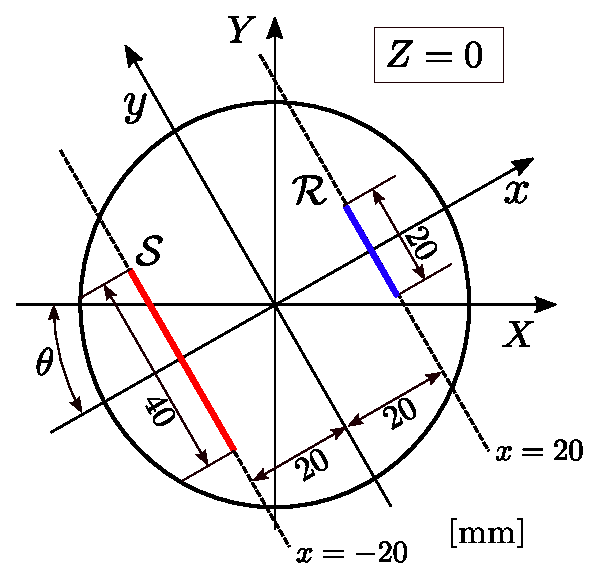
\includegraphics[width=0.5\linewidth]{Figs/fig4.eps} 
	\end{center}
	\caption{
		花崗岩コア供試体の上面における超音波送受信位置の配置.
		${\cal S}$は,ラインフォーカス探触子のカップリング位置を,
		${\cal R}$は,レーザー振動計による計測の測線を表す.
	} 
	\label{fig:fig4}
\end{figure}
%--------------------

